\documentclass{article}

\usepackage{enumerate}
\usepackage{amsmath}
\usepackage{amssymb}
\usepackage{amsfonts}
\usepackage{mathtools}
\usepackage{graphicx}
\usepackage{float}
\usepackage{caption}
\usepackage{subcaption}
\usepackage{color}
\usepackage{relsize}
\usepackage{algpseudocode}
\usepackage[procnames]{listings}
\usepackage[colorlinks = true, allcolors = blue]{hyperref}
\usepackage[]{units}
\usepackage{framed}
\usepackage{breqn}
\usepackage{lipsum}
\usepackage{algorithm}
\usepackage{algpseudocode}
\usepackage{fancyhdr}
\usepackage{extramarks}
\usepackage{xfrac}
\usepackage{multicol}
\usepackage{bibentry}
\usepackage{verbatim}
\nobibliography*

\def\arraystretch{1.2}

\topmargin = -0.45in
\evensidemargin = 0in
\oddsidemargin = 0in
\textwidth = 6.5in
\textheight = 9.0in
\headsep = 0.25in

\pagestyle{fancy}
\lhead{Pedro D. Bello-Maldonado}
\chead{}
\rhead{Research notes}
\lfoot{IBM Research - Sustainability}
\cfoot{\thepage}
\rfoot{\today}

\renewcommand\headrulewidth{0.4pt}
\renewcommand\footrulewidth{0.4pt}

\renewcommand{\algorithmicrequire}{\textbf{Input:}}
\renewcommand{\algorithmicensure}{\textbf{Output:}}
\renewcommand{\algorithmicforall}{\textbf{parallel for}}

\setlength{\parindent}{0pt}
\setlength{\parskip}{5pt plus 1pt minus 1pt}

\begin{document}
    \section*{Simple Model - Breakdown}
    {
        \subsection*{Reduced data}
        {
            \begin{figure}[H]
                \centering
                \begin{subfigure}[]{0.45 \textwidth}
                    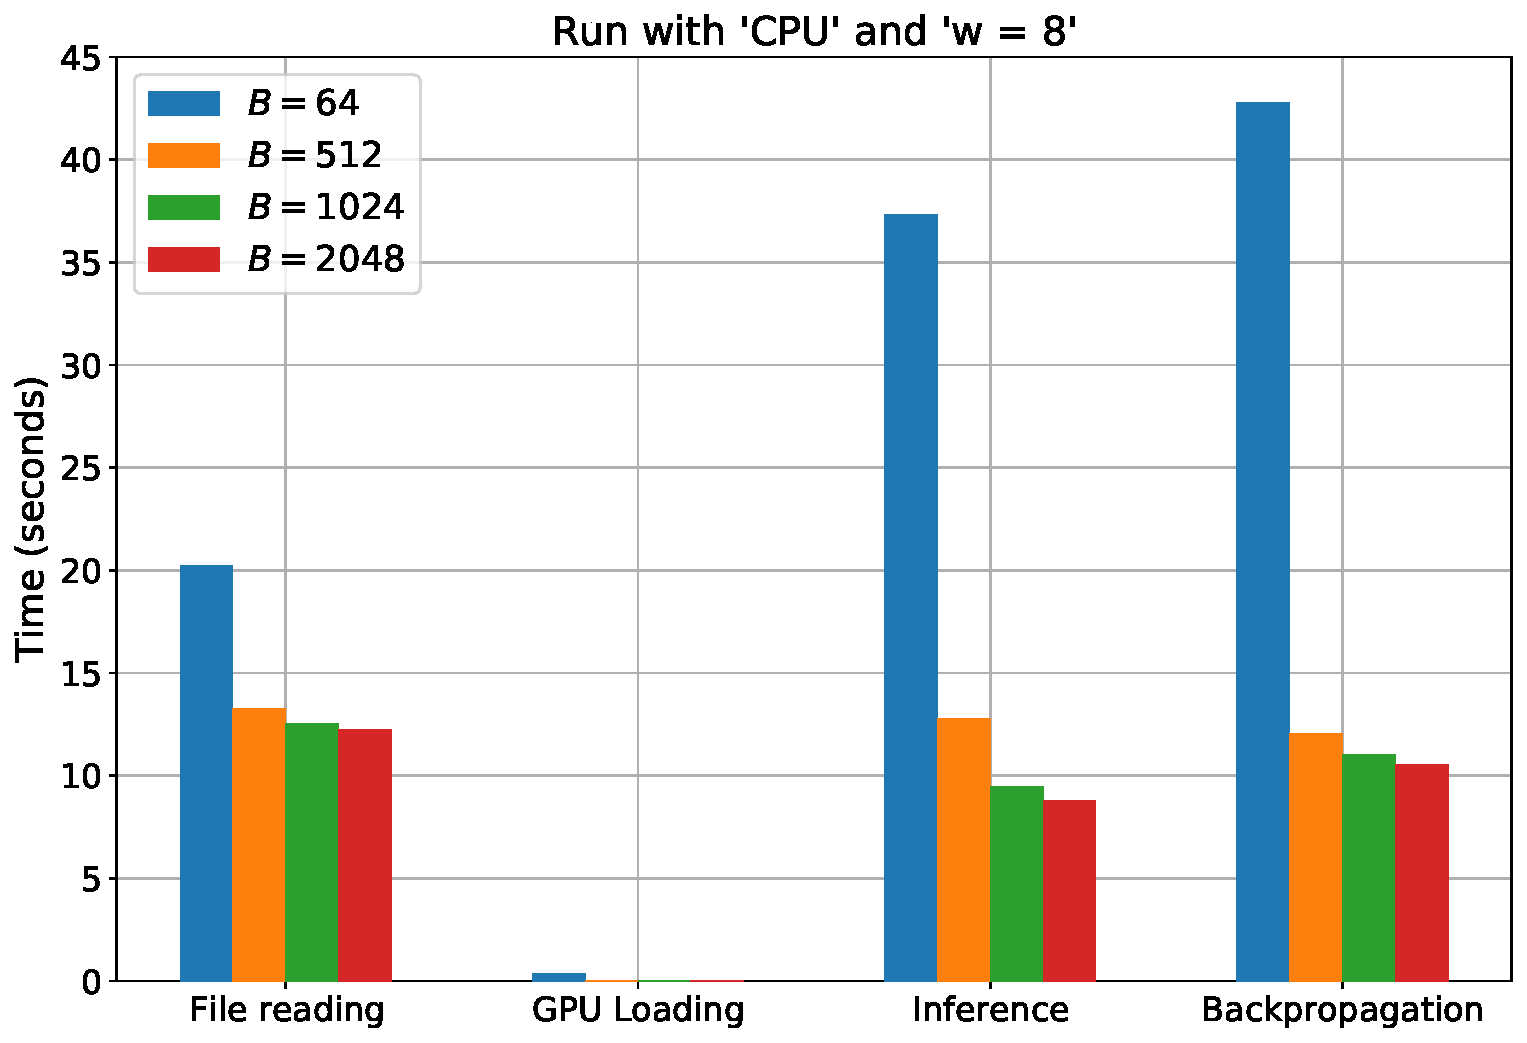
\includegraphics[width = 1.0 \textwidth]{Figures/cpu_8x8_reduced.pdf}
                    \caption{CPU}
                \end{subfigure}
                \begin{subfigure}[]{0.45 \textwidth}
                    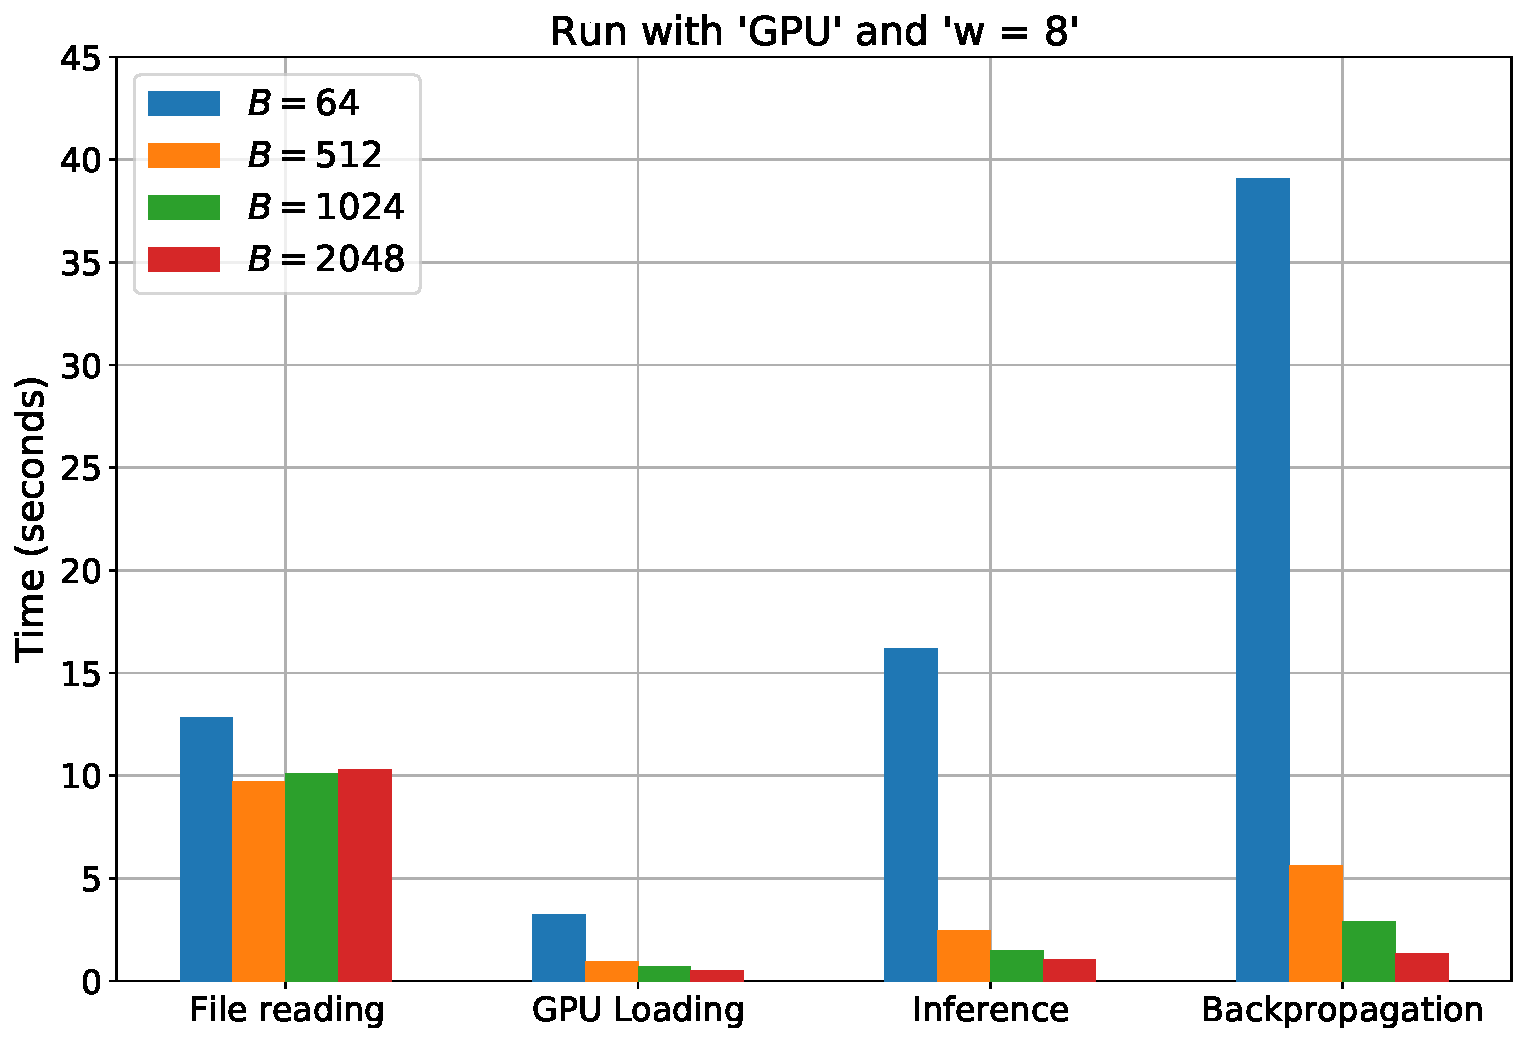
\includegraphics[width = 1.0 \textwidth]{Figures/gpu_8x8_reduced.pdf}
                    \caption{GPU}
                \end{subfigure}
                \caption{8x8 training images}
            \end{figure}

            \begin{figure}[H]
                \centering
                \begin{subfigure}[]{0.45 \textwidth}
                    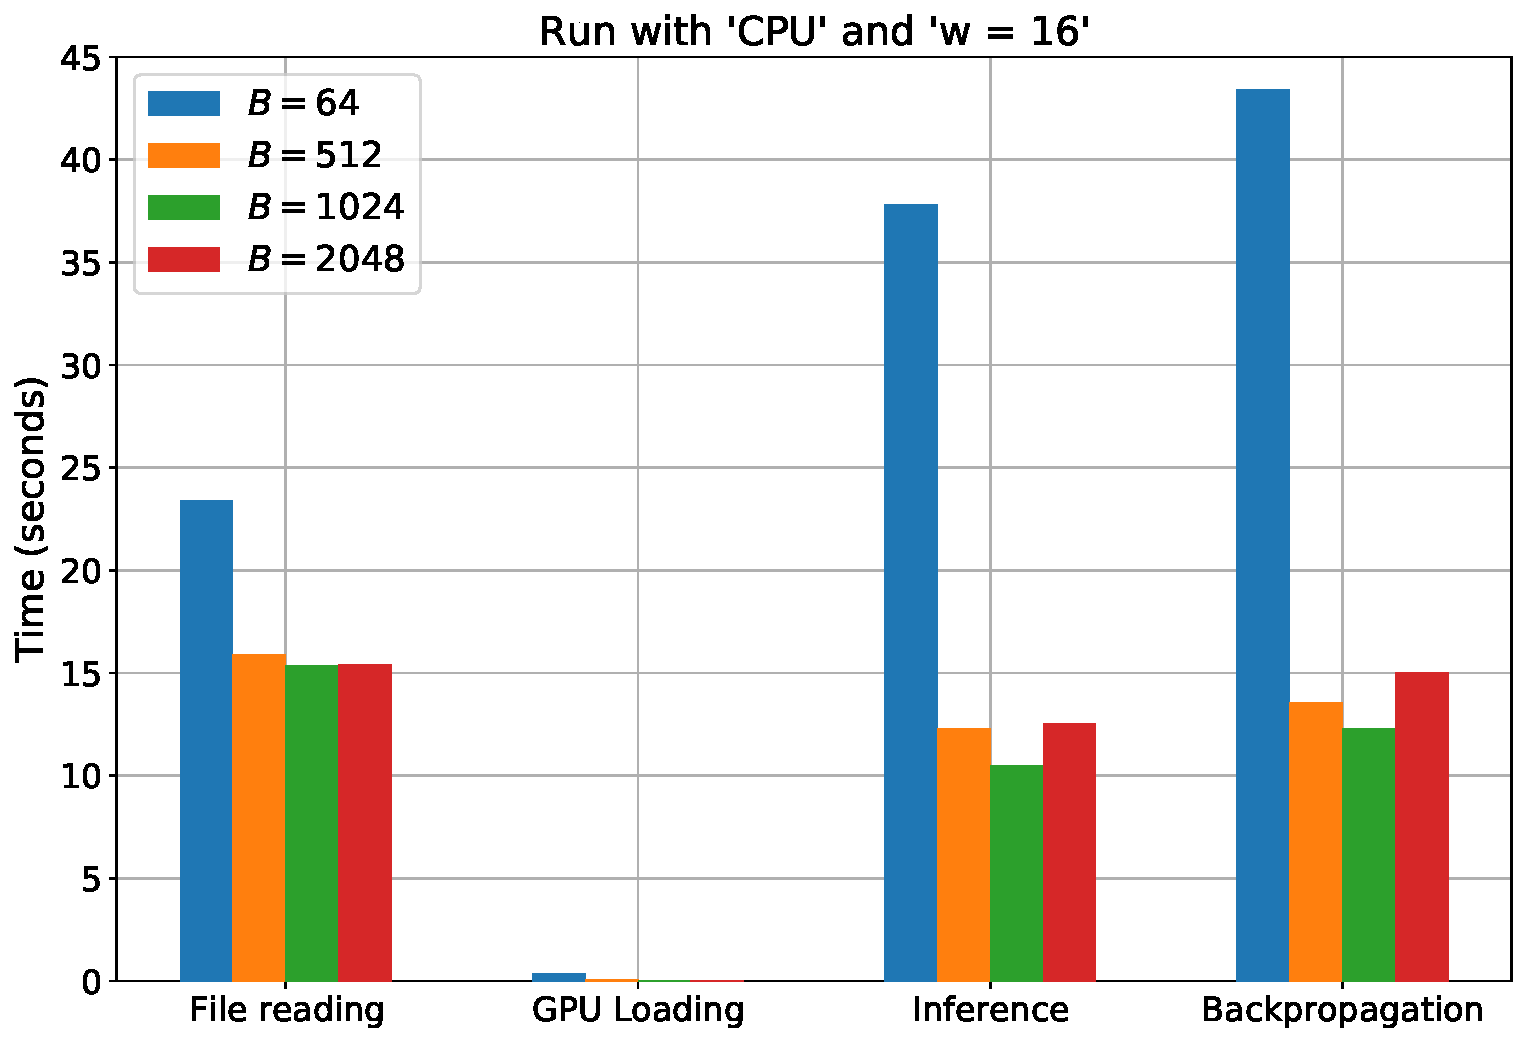
\includegraphics[width = 1.0 \textwidth]{Figures/cpu_16x16_reduced.pdf}
                    \caption{CPU}
                \end{subfigure}
                \begin{subfigure}[]{0.45 \textwidth}
                    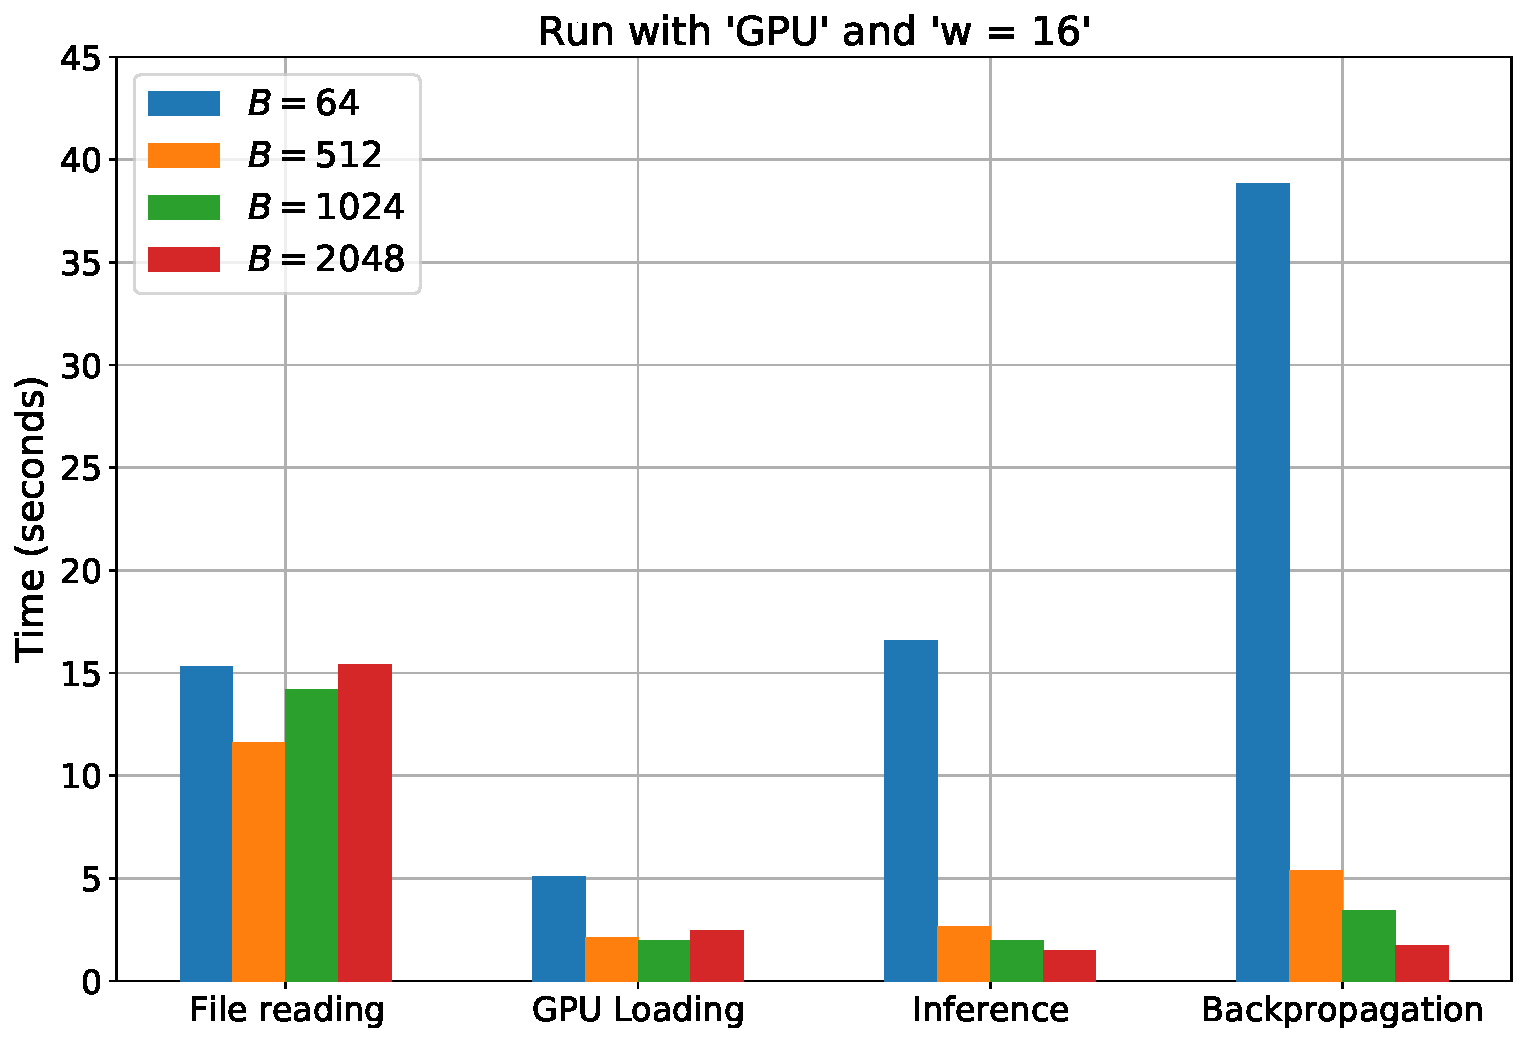
\includegraphics[width = 1.0 \textwidth]{Figures/gpu_16x16_reduced.pdf}
                    \caption{GPU}
                \end{subfigure}
                \caption{16x16 training images}
            \end{figure}
        }

        \subsection*{Full data}
        {
            \begin{figure}[H]
                \centering
                \begin{subfigure}[]{0.45 \textwidth}
                    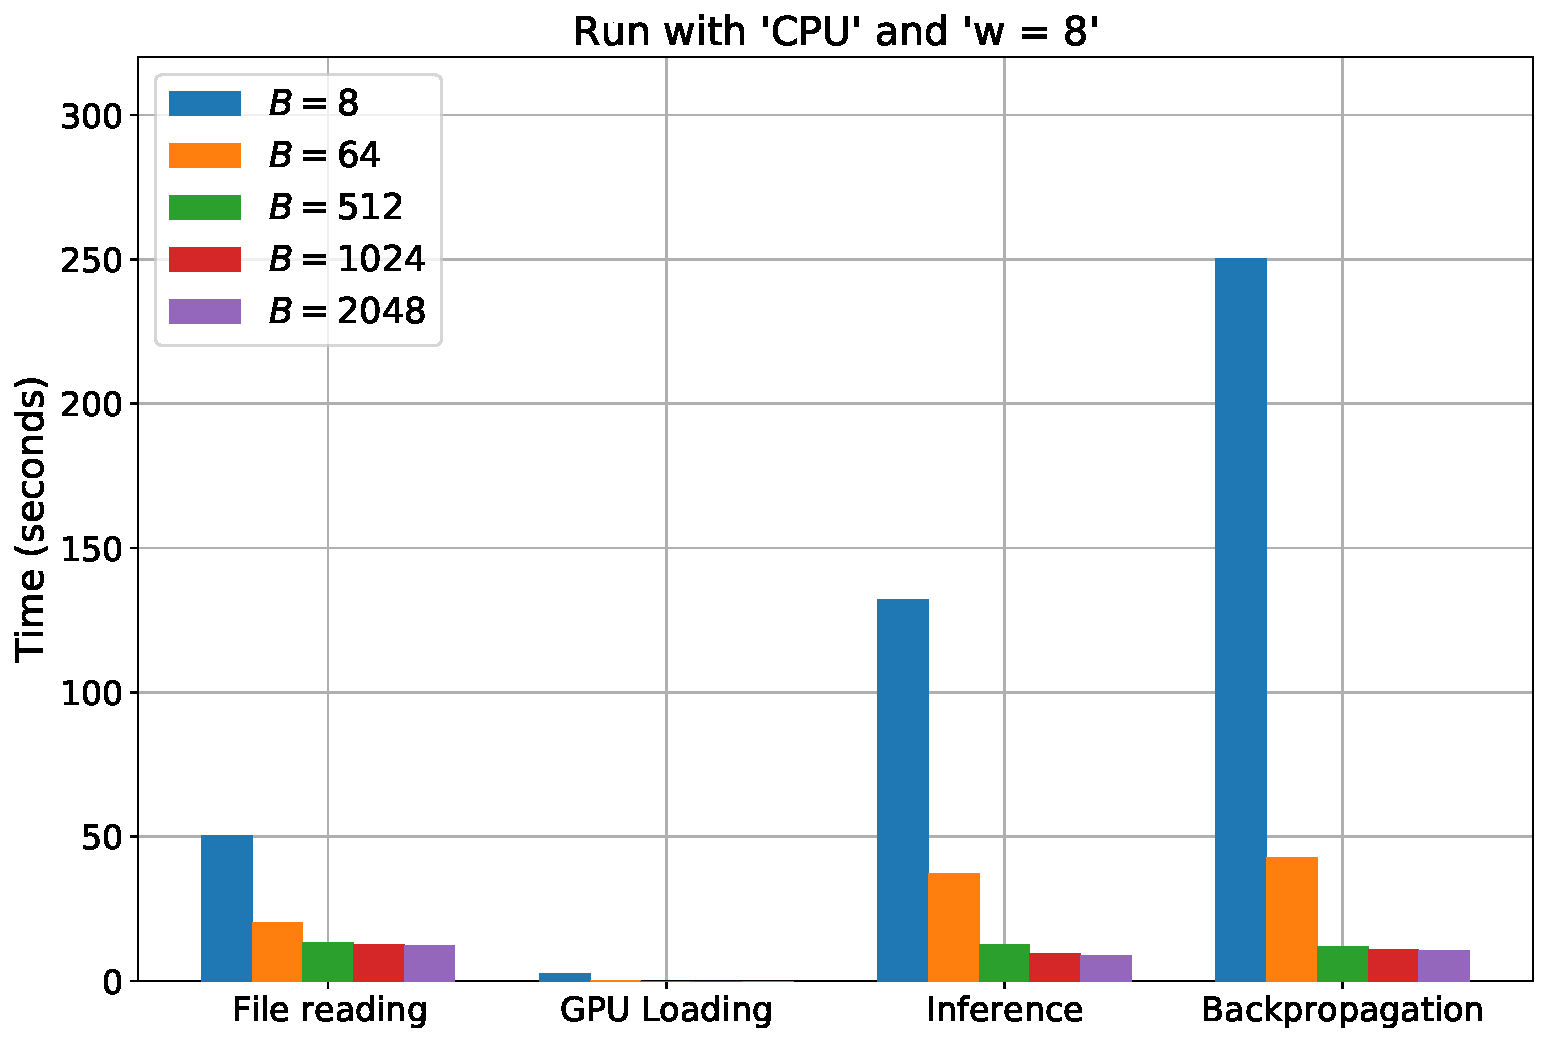
\includegraphics[width = 1.0 \textwidth]{Figures/cpu_8x8_full.pdf}
                    \caption{CPU}
                \end{subfigure}
                \begin{subfigure}[]{0.45 \textwidth}
                    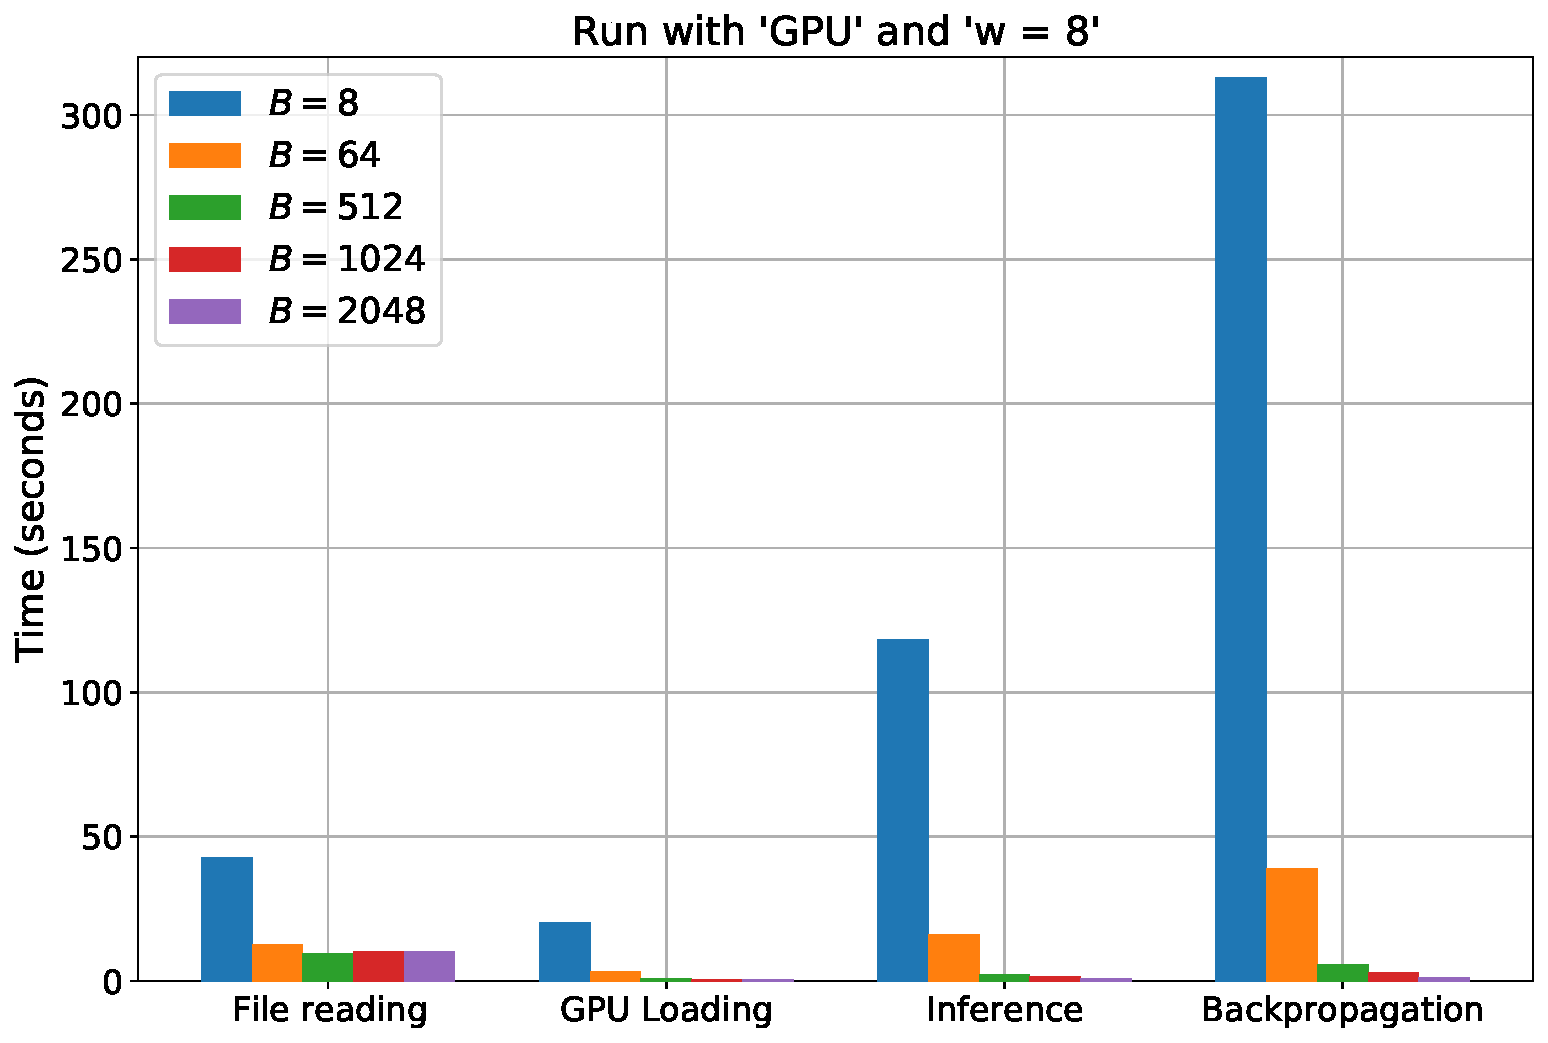
\includegraphics[width = 1.0 \textwidth]{Figures/gpu_8x8_full.pdf}
                    \caption{GPU}
                \end{subfigure}
                \caption{8x8 training images}
            \end{figure}

            \begin{figure}[H]
                \centering
                \begin{subfigure}[]{0.45 \textwidth}
                    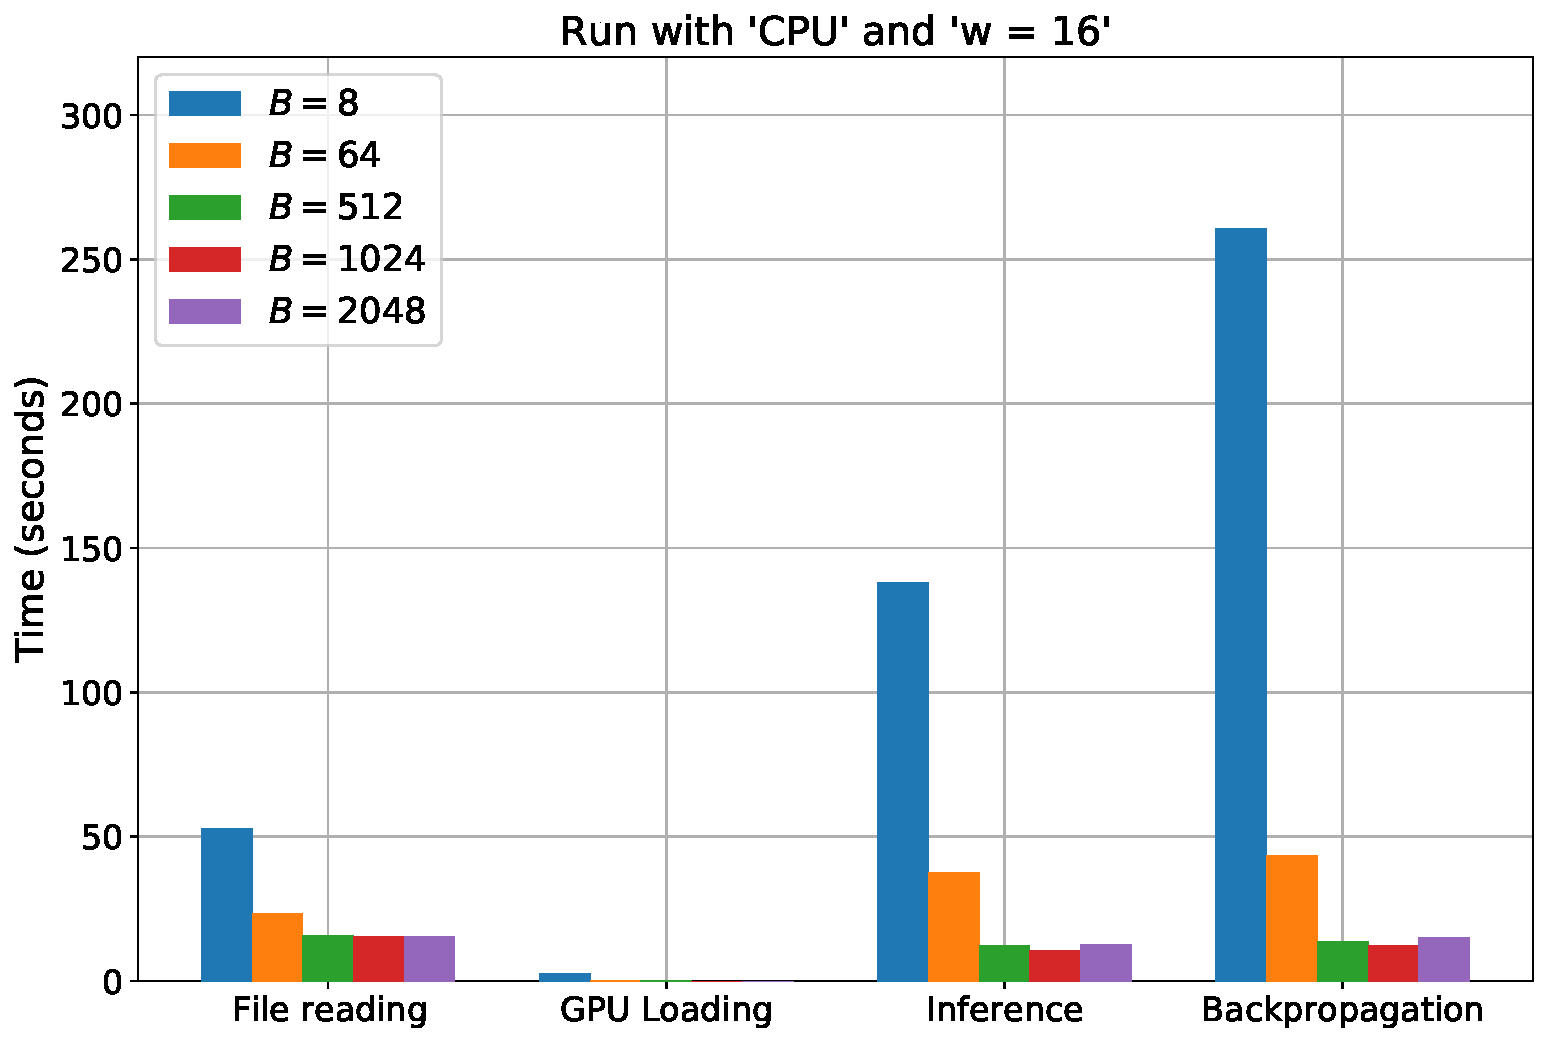
\includegraphics[width = 1.0 \textwidth]{Figures/cpu_16x16_full.pdf}
                    \caption{CPU}
                \end{subfigure}
                \begin{subfigure}[]{0.45 \textwidth}
                    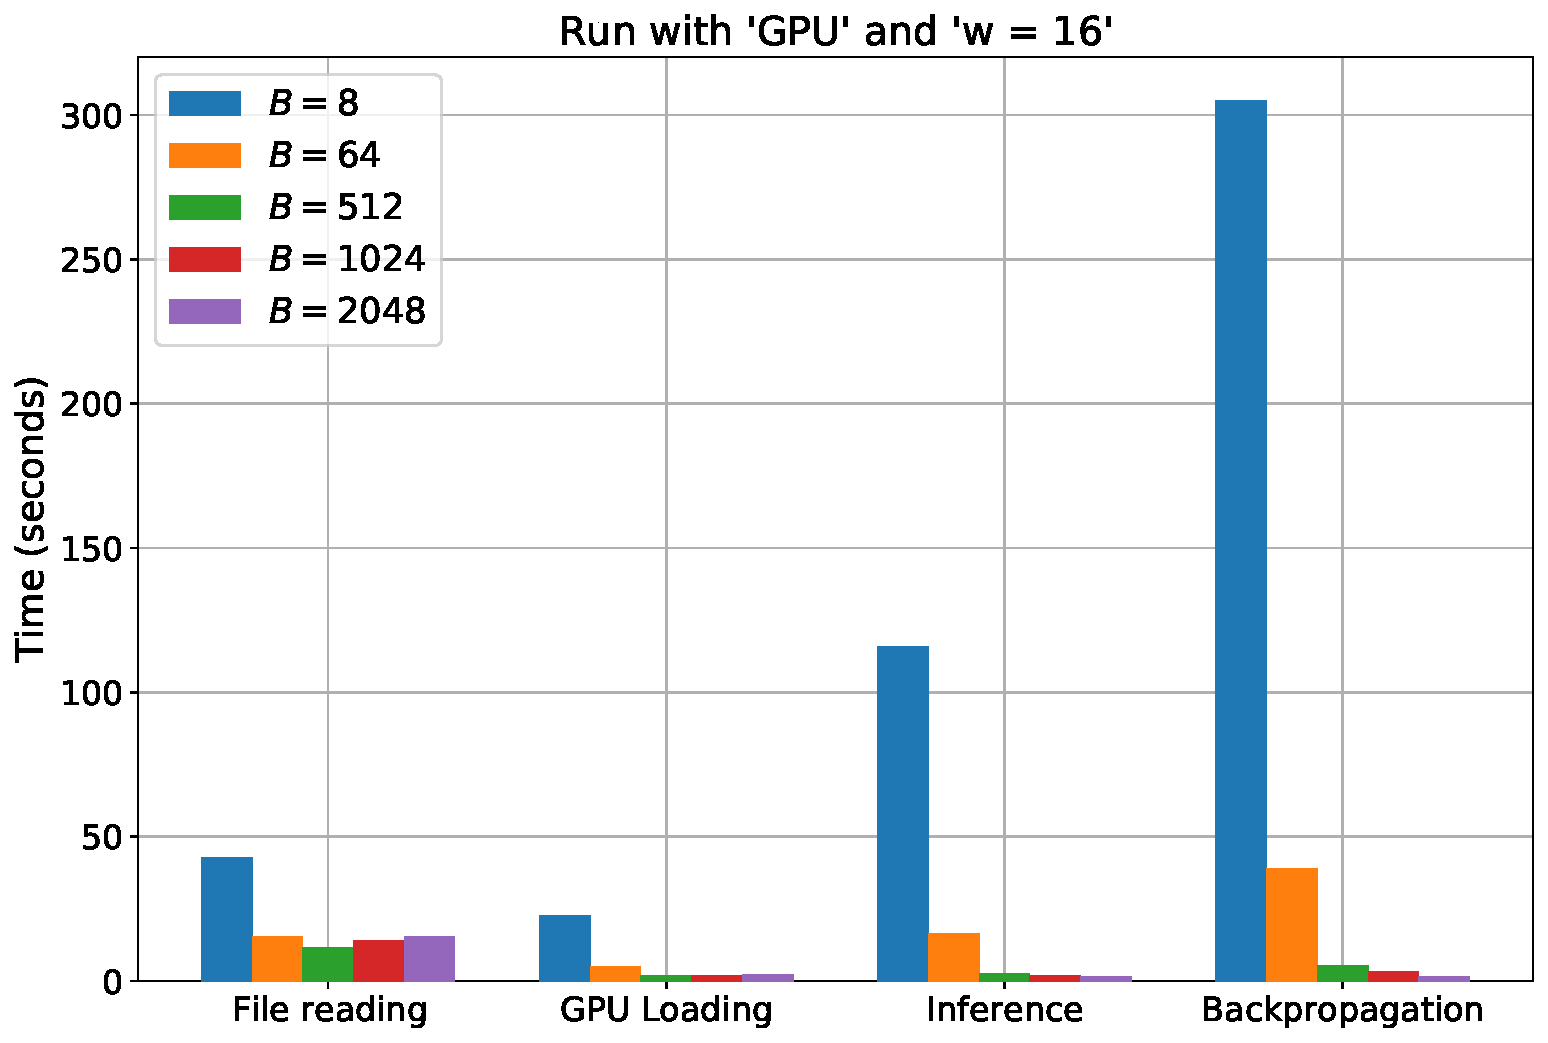
\includegraphics[width = 1.0 \textwidth]{Figures/gpu_16x16_full.pdf}
                    \caption{GPU}
                \end{subfigure}
                \caption{16x16 training images}
            \end{figure}
        }
    }
\end{document}
